% Editable source for online_path.pdf (pdflatex online_path.tex; pdftoppm -png -r 150 -singlefile online_path.pdf online_path).
% Where canonicalization sits in the n=83 one-target IC online interval (crypto 770f6a69
% examples/koblitz_orbit_dlp_fast_online.rs, wide path, scan_state128), and in the E-1 stage.
% Counts: reconcile run 38617911080, iB770c on Q0 (probes, root calls, relation checks, phase times).
\documentclass[tikz,border=6pt]{standalone}
\usepackage[T1]{fontenc}
\usetikzlibrary{positioning,arrows.meta,fit,backgrounds}
\begin{document}
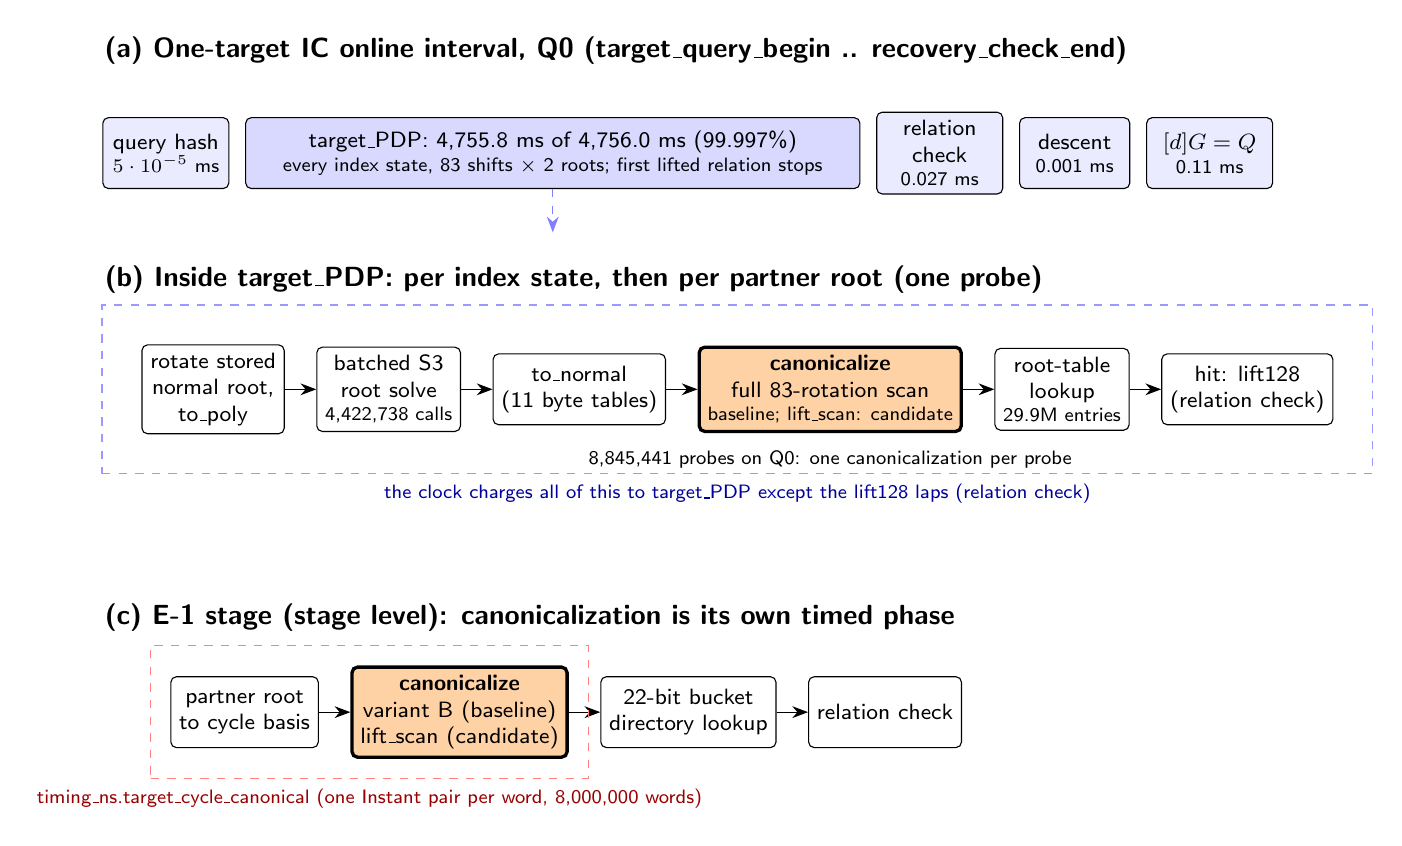
\begin{tikzpicture}[font=\sffamily\footnotesize,
  box/.style={draw,rounded corners=2pt,align=center,minimum height=9mm,inner sep=3pt},
  hot/.style={box,fill=orange!35,very thick},
  ph/.style={box,fill=blue!8},
  >={Stealth[length=2mm]}]
\node[font=\sffamily\bfseries,anchor=west] at (-0.3,1.3) {(a) One-target IC online interval, Q0 (target\_query\_begin .. recovery\_check\_end)};
\node[ph,minimum width=16mm] (q) at (0.6,0) {query hash\\[-1pt]\scriptsize $5\cdot10^{-5}$ ms};
\node[ph,minimum width=78mm,right=2mm of q,fill=blue!15] (pdp) {target\_PDP: 4,755.8 ms of 4,756.0 ms (99.997\%)\\[-1pt]\scriptsize every index state, 83 shifts $\times$ 2 roots; first lifted relation stops};
\node[ph,minimum width=16mm,right=2mm of pdp] (rc) {relation\\check\\[-1pt]\scriptsize 0.027 ms};
\node[ph,minimum width=14mm,right=2mm of rc] (de) {descent\\[-1pt]\scriptsize 0.001 ms};
\node[ph,minimum width=16mm,right=2mm of de] (vc) {$[d]G=Q$\\[-1pt]\scriptsize 0.11 ms};
\node[font=\sffamily\bfseries,anchor=west] at (-0.3,-1.6) {(b) Inside target\_PDP: per index state, then per partner root (one probe)};
\node[box] (rot) at (1.2,-3.0) {rotate stored\\normal root,\\to\_poly};
\node[box,right=4mm of rot] (s3) {batched S3\\root solve\\[-1pt]\scriptsize 4,422,738 calls};
\node[box,right=4mm of s3] (tn) {to\_normal\\(11 byte tables)};
\node[hot,right=4mm of tn] (cn) {\textbf{canonicalize}\\full 83-rotation scan\\[-1pt]\scriptsize baseline; lift\_scan: candidate};
\node[box,right=4mm of cn] (lk) {root-table\\lookup\\[-1pt]\scriptsize 29.9M entries};
\node[box,right=4mm of lk] (lf) {hit: lift128\\(relation check)};
\draw[->] (rot) -- (s3); \draw[->] (s3) -- (tn);
\draw[->] (tn) -- (cn); \draw[->] (cn) -- (lk); \draw[->] (lk) -- (lf);
\node[below=1mm of cn,font=\sffamily\scriptsize,align=center] {8,845,441 probes on Q0: one canonicalization per probe};
\begin{scope}[on background layer]
\node[draw=blue!40,dashed,fit=(rot)(lf),inner sep=5mm,label={[font=\sffamily\scriptsize,blue!60!black]below:the clock charges all of this to target\_PDP except the lift128 laps (relation check)}] {};
\end{scope}
\draw[->,blue!50,dashed] (pdp.south) -- ++(0,-0.55);
\node[font=\sffamily\bfseries,anchor=west] at (-0.3,-5.9) {(c) E-1 stage (stage level): canonicalization is its own timed phase};
\node[box] (e1) at (1.6,-7.1) {partner root\\to cycle basis};
\node[hot,right=4mm of e1] (e2) {\textbf{canonicalize}\\variant B (baseline)\\lift\_scan (candidate)};
\node[box,right=4mm of e2] (e3) {22-bit bucket\\directory lookup};
\node[box,right=4mm of e3] (e4) {relation check};
\draw[->] (e1) -- (e2); \draw[->] (e2) -- (e3); \draw[->] (e3) -- (e4);
\node[draw=red!50,dashed,fit=(e1)(e2),inner sep=2.5mm,label={[font=\sffamily\scriptsize,red!60!black]below:timing\_ns.target\_cycle\_canonical (one Instant pair per word, 8,000,000 words)}] {};
\end{tikzpicture}
\end{document}
